% !TeX program = lualatex
\documentclass[tikz,border=6pt]{standalone}

\usepackage{tikz}
\usetikzlibrary{calc,angles,quotes}

\begin{document}
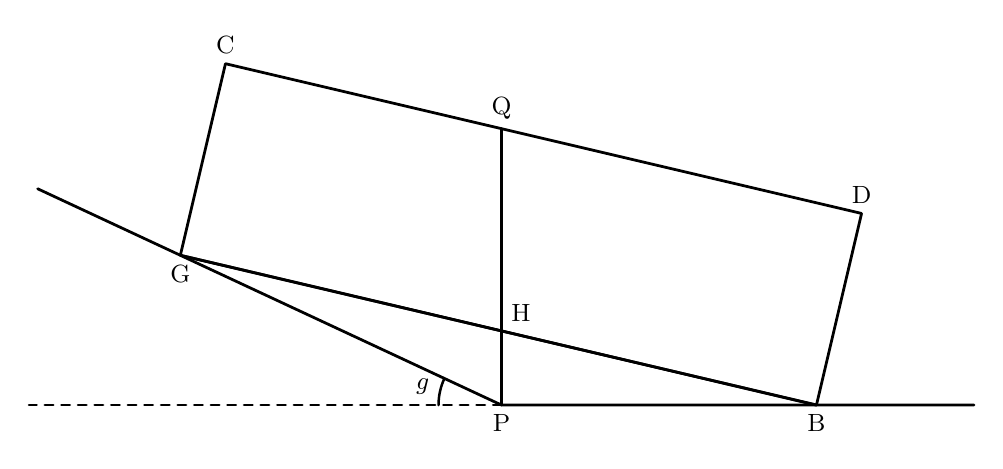
\begin{tikzpicture}[x=1cm,y=1cm, line cap=round, line join=round, font=\small]

% =========================
% 1) THAM SỐ HÓA (đổi ở đây)
% =========================
\def\alpha{25}   % góc dốc của mặt đường (độ)
\def\Lext{6}   % độ dài phần đường ngang (từ P sang phải)
\def\Lback{6.5}  % độ dài kéo dài đường dốc về bên trái (từ P)
\def\b{4}      % tọa độ x của B (B nằm trên mặt đường ngang y=0)
\def\tG{4.5}     % khoảng cách từ P đi lên-trái trên dốc để tới G
\def\h{2.5}      % chiều cao thùng xe (vuông góc với GB)

% =========================
% 2) TIỀN TÍNH TOÁN (tránh lỗi calc)
% =========================
\pgfmathsetmacro{\dxBack}{-\Lback*cos(\alpha)}
\pgfmathsetmacro{\dyBack}{ \Lback*sin(\alpha)}

\pgfmathsetmacro{\Gx}{-\tG*cos(\alpha)}
\pgfmathsetmacro{\Gy}{ \tG*sin(\alpha)}

\pgfmathsetmacro{\dxPleft}{-1.2*cos(\alpha)}
\pgfmathsetmacro{\dyPleft}{ 1.2*sin(\alpha)}

% =========================
% 3) ĐIỂM MỐC: P là gốc
% =========================
\coordinate (P) at (0,0);
\coordinate (G) at (\Gx,\Gy);
\coordinate (B) at (\b,0);

% =========================
% 4) DỰNG HÌNH CHỮ NHẬT G-C-D-B
%    (đáy là GB, cạnh bên vuông góc với GB)
% =========================
% véc-tơ w = B - G
\pgfmathsetmacro{\wx}{\b - \Gx}
\pgfmathsetmacro{\wy}{0 - \Gy}
\pgfmathsetmacro{\Lw}{sqrt(\wx*\wx+\wy*\wy)}

% pháp tuyến đơn vị n = (-wy, wx)/|w|
\pgfmathsetmacro{\nx}{-(\wy)/\Lw}
\pgfmathsetmacro{\ny}{ (\wx)/\Lw}

% C = G + h n,  D = B + h n
\pgfmathsetmacro{\Cx}{\Gx + \h*\nx}
\pgfmathsetmacro{\Cy}{\Gy + \h*\ny}
\pgfmathsetmacro{\Dx}{\b  + \h*\nx}
\pgfmathsetmacro{\Dy}{0   + \h*\ny}
\coordinate (C) at (\Cx,\Cy);
\coordinate (D) at (\Dx,\Dy);

% =========================
% 5) Q là giao của CD với đường thẳng đứng x=0
% =========================
\pgfmathsetmacro{\tQ}{(0-\Cx)/(\Dx-\Cx)}
\pgfmathsetmacro{\Qx}{\Cx + \tQ*(\Dx-\Cx)}
\pgfmathsetmacro{\Qy}{\Cy + \tQ*(\Dy-\Cy)}
\coordinate (Q) at (\Qx,\Qy);

% 6) H là giao của GB với x=0
\pgfmathsetmacro{\tH}{(0-\Gx)/(\b-\Gx)}
\pgfmathsetmacro{\Hx}{\Gx + \tH*(\b-\Gx)}
\pgfmathsetmacro{\Hy}{\Gy + \tH*(0-\Gy)}
\coordinate (H) at (\Hx,\Hy);

% =========================
% 7) VẼ THEO KHỐI
% =========================
% Mặt đường: dốc + ngang
\draw[line width=1.0pt] ($(P)+(\dxBack,\dyBack)$) -- (P) -- ($(P)+(\Lext,0)$);

% Mặt đường: dốc + ngang
\draw[dashed, line width=1.0pt] (P) -- ($(P)-(\Lext,0)$);
% Thùng xe
\draw[line width=1.0pt] (G) -- (C) -- (D) -- (B) -- cycle;

% Đường chéo GB
\draw[line width=1.0pt] (G) -- (B);

% Đường thẳng đứng qua Q xuống P
\draw[line width=1.0pt] (Q) -- (P);

% =========================
% 8) KÝ HIỆU / NHÃN
% =========================
% Góc alpha tại P
\coordinate (Pright) at ($(P)+(1.2,0)$);
\coordinate (Pleft)  at ($(P)+(\dxPleft,\dyPleft)$);
\draw pic[draw, angle radius=0.65, angle eccentricity=1.25] {angle = Pright--P--Pleft};

% Nhãn điểm
\node[above] at (C) {C};
\node[above] at (D) {D};
\node[below] at (G) {G};
\node[below] at (B) {B};
\node[above] at (Q) {Q};
\node[above right] at (H) {H};
\node[below] at (P) {P};

% ------------------------------------------------------
% Góc g giữa dốc và mặt đường

\coordinate (Xroad) at ($(P)-(1,0)$);
% điểm xác định hướng mặt đường

\coordinate (Xslope) at ($(P)+(-1,{tan(\alpha)})$);
% điểm xác định hướng dốc

\pic[draw, line width=0.9pt, angle radius=8mm]
  {angle=Xslope--P--Xroad};

\node at ($(P)+(-1,{tan(\alpha)/2})$) {$g$};

\end{tikzpicture}
\end{document}
